\chapter{Methods and Materials}
\section{Wastewater treatment plant description}
\subsection{Process and data sources in SWHEPP}
Shek Wu Hui Effluent Polish Plant (SWHEPP) is a secondary sewage treatment plant, which treats the municipal wastewater of the Sheung Shui, Fanling Districts and adjacent areas, and treated leachate effluent from North East New Territories (NENT) leachate treatment plant. The plant is designed for 300,000 population equivalents (PE) in 2001, and in 2009, the daily treatment capacity has been expanded from 80,000 m$^3$/day to 93,000 m$^3$/day. SHWEPP is operated and maintained by Drainage Services Department (DSD), and the plant will be upgraded to teritary treatment level to increase the treatment capacity of 190,000 m$^3$/day by the end of 2025. As shown in Fig.~\ref{fig:SHWEPP-flowchart}, the treatment plant is mainly comprised of primary sedimentation, secondary biological treatment, and final sedimentation followed by a membrane bioreactor (MBR), which provides an advanced level of organic and suspended solids removal. To monitor the effluent quality in real-time, low volume of the MBR effluent is pumped to an effluent container near by the MBR location. Two on-line meters, ammoniacal nitrogen on-line sensor and colour level on-line analyzer are installed in the effluent container, which are indicated as (a) and (b) in Fig.~\ref{fig:SHWEPP-flowchart}.

\begin{figure}[h]
    \centering
    \includegraphics[width=0.9\columnwidth]{imgs/Sewage-treatment-process-flowchart.png}
    \caption{Sewage treatment process flowchart at SWHEPP (adapted from Drainage Services Department 2020)}
    \label{fig:SHWEPP-flowchart}
\end{figure}

\subsection{Reclaimed water standard}
Reclaimed water for non-potable reuses can serve for irrigation for agricultures, toilet flushing and irrigation for landscaping, etc. Water Supply Department (WSD) will soon implement a reclaimed water supply system in SWHEPP by disinfecting the teriary treated sewage (i.e., MBR permeate). The produced reclaimed water will be served for non-potable reuses and is required to satisfy the water quality standards, shown in Table.~\ref{tab:reclaimed-standard}.

\begin{table}[!ht]
    \centering
    \caption{\label{tab:reclaimed-standard}Endorsed Reclaimed Water Quality Standards from Water Supply Department.}
    \begin{NiceTabular}{lcl}
        \toprule
        Parameter & Unit & Requirement \tabularnote{The water quality standards for all parameters are applicable at the point-of-use of the system.} \\
        \midrule
        \textit{E. coli} & cfu/100 mL & Not detectable \\ 
        Colour & Hazen Unit & $\le$ 20 \\ 
        Ammoniacal Nitrogen (NH$_3$-N) & mg/L as N & $\le$ 1 \\ 
        Total Residual Chlorine & mg/L & $\ge$ 0.2 \\ 
        Dissolved Oxygen & mg/L & $\ge$ 0.2 \\ 
        Turbidity & NTU & $\le$ 5 \\ 
        5-day Biochemical Oxygen Demand & mg/L & $\le$ 1 \\ 
        pH & - & 6-9 \\ 
        Threshold Odour Number & - & $\le$ 100 \\ 
        Synthetic detergents & mg/L & $\le$ 5 \\
        \bottomrule
    \end{NiceTabular}
\end{table}

\section{Data collection and preparation}

\begin{figure}[h]
    \centering
    \includegraphics[width=0.8\columnwidth]{imgs/instrument/sampling-tank.png}
    \caption{Colour levels and ammonia concentration are measure in the effluent container (i.e., on the right of the image.) A water pump transports MBR effluent to the effluent container continuously at real-time. The black vault on the left of the image contains a laptop and a colour spectrophotometer.} 
    \label{fig:sampling-tank}
 \end{figure}

\subsection{Ammonia data monitoring and collection}
To enable us to perform on-line monitoring of ammonium concentration (NH$_{3}$-N) in the MBR effluent, a Ammonium and Potassium Probe, AmmoLyt$^\circledR$Plus 700 IQ (Xylem Company) is installed as in Fig.~\ref{fig:nh3-sensor-a} in the effluent container, as shown in Fig.~\ref{fig:sampling-tank}. The operation was commenced on 27 April 2021 and completed on 27 March 2022. The ion-selective electrode (ISE) probe provides continuous and reagentless monitoring of ammonium and potassium at the configured interval of one measurement per minute. Due to the ISE probe cannot differentiate the potentials difference cause by ammonium and potassium ions in the electrodes, the on-line monitoring of ammonium concentration requires the continuous calibration using potassium concentration.

The instrument records ammonium concentration as NH$_{4}$-N mg/L, a form to express the sum of nitrogen found in reduced nitrogen (III) form. Ammonia has a reported pKa of 9.25 \citep{nationalcenterforbiotechnologyinformationPubChemCompoundSummary2022}, meaning ammonium is a primary species under the pH of 9.25 in water. In WWTPs, the pH in water normally ranges from pH of 7--8, making the NH$_{4}$-N concentration the dominant species. Both ammonia and ammonium contain one nitrogen atom, 1 mg/L NH$_{3}$-N is the same as 1 mg/L NH$_{4}$-N. Thus, to prevent confusion, in the following paragraph the unit of NH$_{4}$-N will be expressed by NH$_{3}$-N, which is the unit used in the water quality standard. The collection of on-line ammonia data is achieved through downloading csv files from the website connected to the IQ Sensor Controller (Xylem Comapny), as shown in Fig.~\ref{fig:nh3-sensor-b}. 

\begin{figure}[h]
    \centering
    \begin{subfigure}{0.3\textwidth}
      \includegraphics[width=\linewidth]{imgs/instrument/ammonium-sensor.png}
      \caption{AmmoLyt$^\circledR$Plus 700 IQ, Xylem} \label{fig:nh3-sensor-a}
    \end{subfigure}%
    \hspace{5em}%   % maximize separation between the subfigures
    \begin{subfigure}{0.3\textwidth}
      \includegraphics[width=\linewidth]{imgs/instrument/controller-for-iq-sensor.png}
      \caption{DIQ/S 284-EF controller, Xylem} \label{fig:nh3-sensor-b}
    \end{subfigure}%  
  \caption{Instrument of on-line ammonium monitoring system.} \label{fig:nh3-sensor}
\end{figure}

\subsection{Color data monitoring and collection}
An hourly monitoring of the colour levels of MBR effluent was conducted from 5 October 2021 to 26 February 2022 by using a custom-made on-line colour analysis system. Originally, the spectrophotometer as Fig.~\ref{fig:hach-sip} and a peristaltic pump as Fig.~\ref{fig:hach-dr3900} can only initiate a single measurement of colour level by pressing the "READ" buttom on the DR3900 panel. To realize continuously sampling and analyzing colour level without human intervention, an actuator with programmable time function was mounted on the panel of DR3900, as shown in Fig.~\ref{fig:hach-actuator}. 

The automatic sampling and analzying of the colour level begins with the action of the actuator, by clicking on the "READ" button to initiate the colour analysis at a fixed interval of 30 minutes. 3 mL of sample was collected from the effluent container and delivered to the spectrophotometer cell. Then, the sample was subsequentially analysed by the spectrophotometer with the data transmitted to an automatic data acquisition and storage software pre-installed in the laptop. The DR3900 device is connected to a laptop, which receives the real-time data and stores on a data management software from Hach company. To access the real-time data from the laptop, Google Remote Desktop is used to operate the laptop via Internet cloud services using any devices having access to the Internet. The entire process is illustrated in Fig.~\ref{fig:diagram-colour-analysis}. After the measurement, the sample will be discharged to the effluent container and the online colour monitoring system is left idle until the next measurement. 

\begin{figure}[h]
    \centering
    \begin{subfigure}{0.3\textwidth}
      \includegraphics[width=\linewidth]{imgs/instrument/SIP10.png}
      \caption{SIP10 peristaltic pump, Hach} \label{fig:hach-sip}
    \end{subfigure}%
    \hspace{2em}   % maximize separation between the subfigures
    \begin{subfigure}{0.3\textwidth}
      \includegraphics[width=\linewidth]{imgs/instrument/DR3900_PS.png}
      \caption{DR3900 spectrophotometer, Hach} \label{fig:hach-dr3900}
    \end{subfigure}%
    \vspace{2em}
    \begin{subfigure}{0.7\textwidth}
        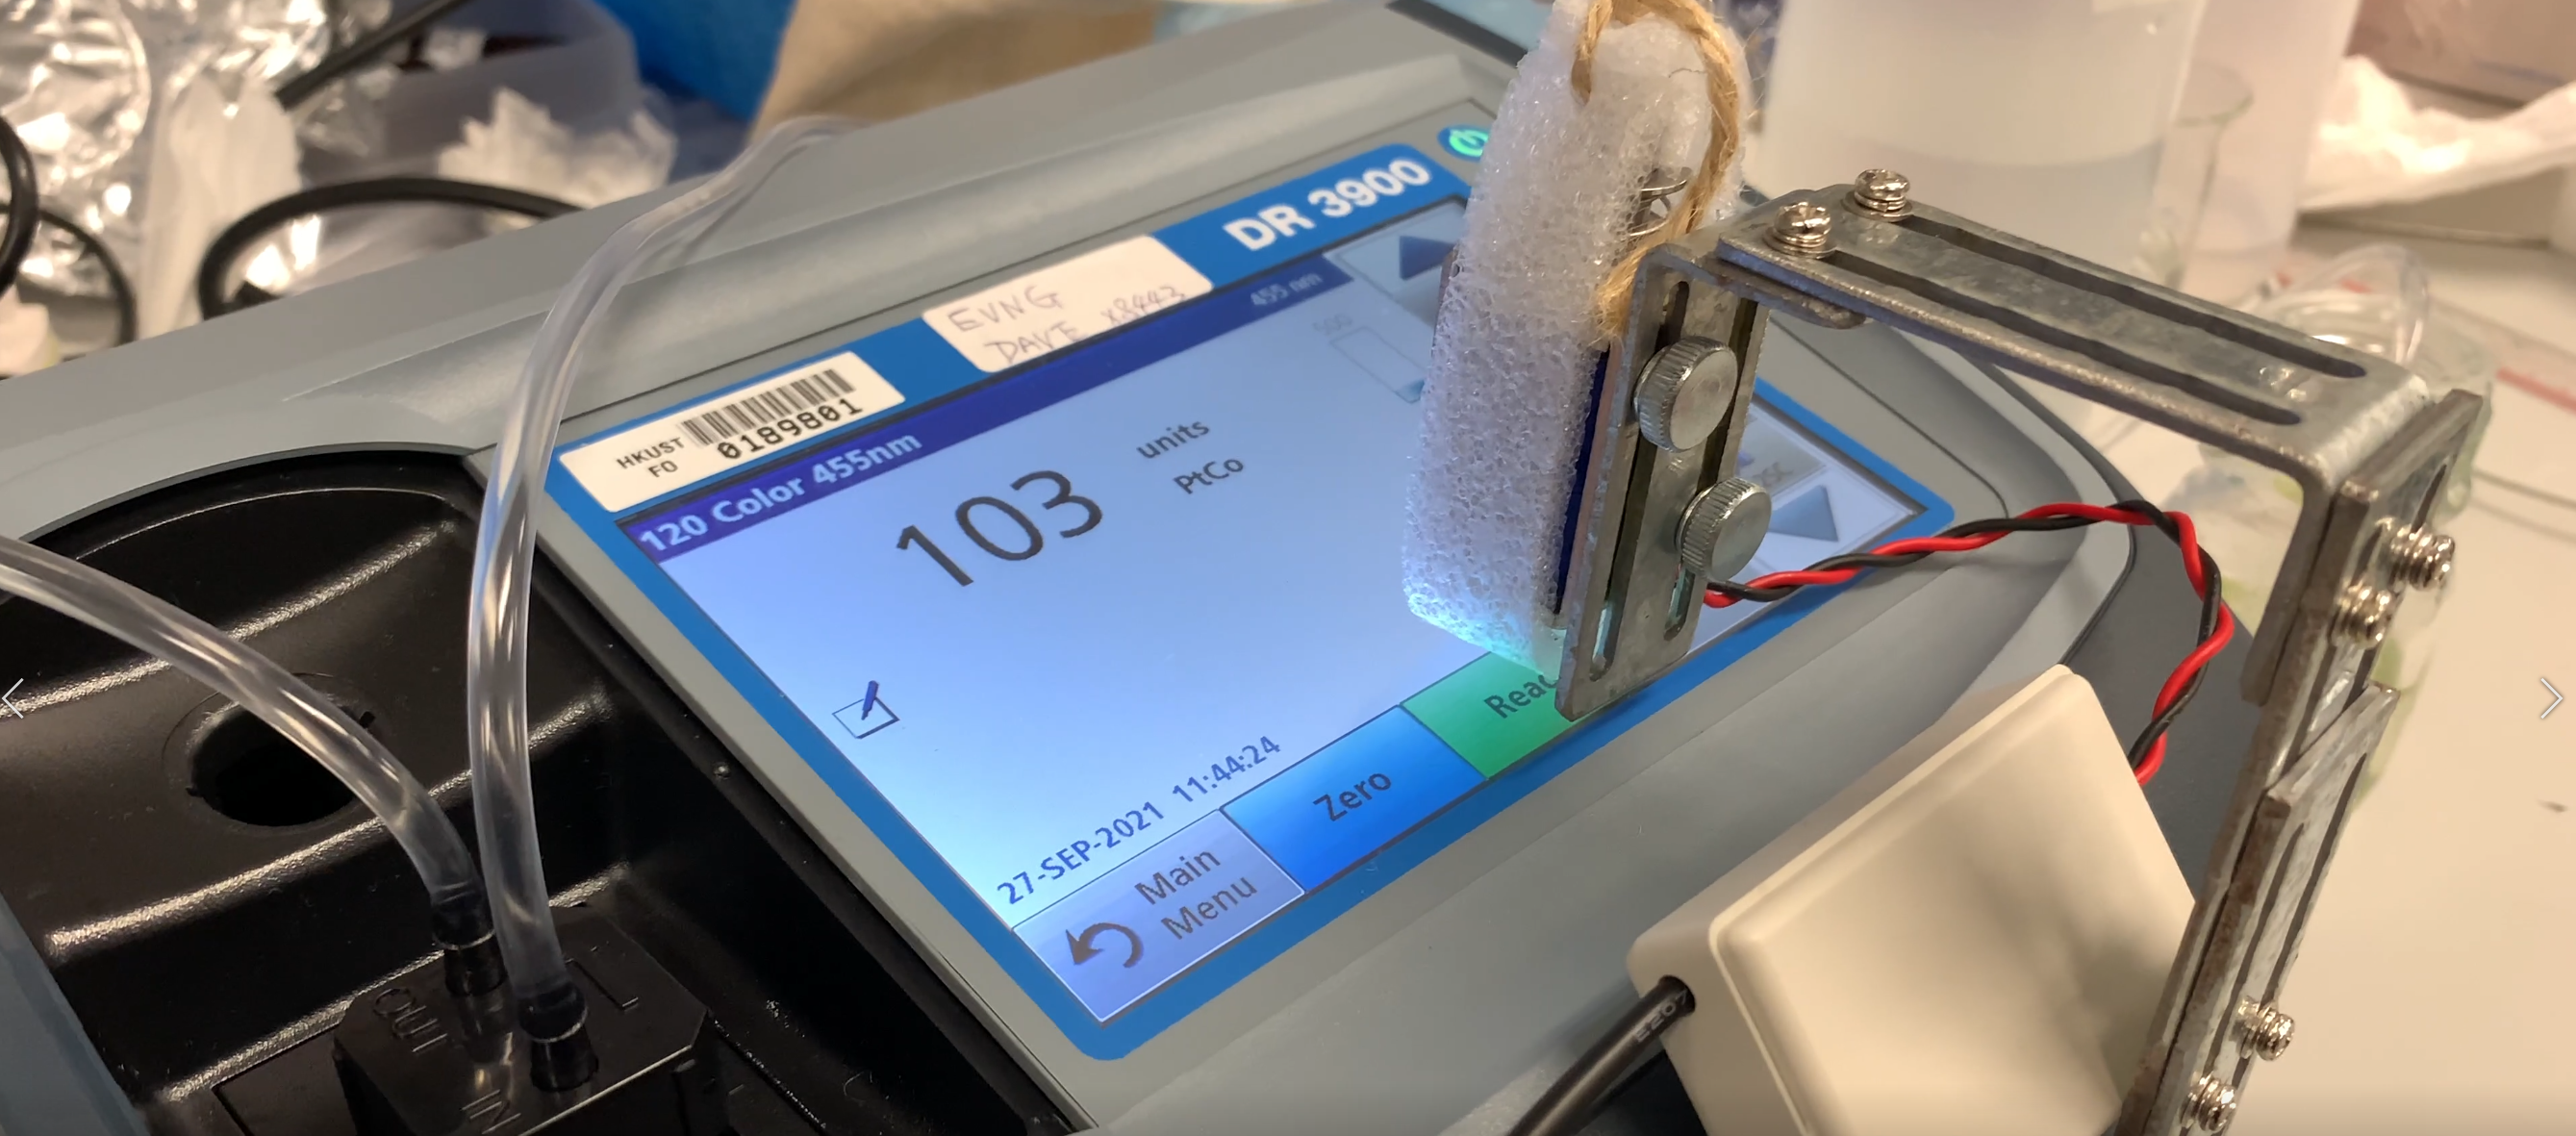
\includegraphics[width=\linewidth]{imgs/instrument/actuator-mount.png}
        \caption{Customized clicker/actuator} \label{fig:hach-actuator}
    \end{subfigure}%  
  \caption{Instruments of on-line colour analysis system.} \label{fig:hach}
\end{figure}

The maintenance and calibration of the DR3900 spectrophotometer is performed on a weekly basis. During the maintenance, the DR3900 device was shut off, and chlorine solution at the concentration of 100 mg/L was pumped into the sampling tubes and the plastic cuvette for disinfection and cleansing. The cleanse of the tubes and cuvette were manually inspected with eyes to make sure no foreign objects were stuck inside. De-ionized water was brought to the site to perform the spectrophotometer calibration after the reboot of DR3900. 

\begin{figure}[h]
    \centering
    \includegraphics[width=0.8\columnwidth]{imgs/instrument/colour-sampler.png}
    \caption{Schematic diagram of the custom-made on-line colour anlaysis system.}
    \label{fig:diagram-colour-analysis}
 \end{figure}

\subsection{Loss function for model evaluation}
Loss functions are used to determine the error between the model outputs (i.e., prediction or forecasting values) and the given target value \citep{deepaiLossFunction2022}. The bigger the difference between the ground truth \boldmath${y}$ and the model outputs \boldmath${\hat{y}}$, the higher the value of the loss function is, meaning the model perfomred poorer. A low value for the loss means the modle perfomred well. The selection of the types of the loss function is essential for training the model to perform specific tasks. In this study, Mean Squared Error (MSE) is used for evaluating the regression models. The values of MSE will never be negative, and is formally defined by the following equation:

\begin{equation}\label{eq-mse}
    MSE=\frac{\sum (y_i-\hat{y_i})^2}{n}
\end{equation}

\subsection{Data cleaning and pre-processing}
The raw data embedded in the original csv files exists many issues, such as missing values, having extreme low or high values, and unreadable texts, etc. Thus, the data cleaning and pre-processing are necessary for more effective process of model training. Python programming language and related modules of Numpy and Pandas were used to clean and pre-process the raw dataset for further usage. The ammonia raw dataset contained 44,640 samples (data points) with 8 variables, giving a matrix size of 44,640 x 8, and the samples were collected in time series at 1 minute interval. The colour level raw dataset contained 1488 samples with 34 variables, giving a matrix size of 1488 x 34, and the samples were collected in time series at 30 minute interval.

Before the high-resolution data from colour and ammonia datasets were compressed into time series data at 1 hour interval via averaging, extreme values were manually removed. For ammonia dataset, we replaced the values higher than 7.0 mg/L with NaN (i.e., Not a number), and futher use interpolation to fill up the NaN along with the missing values in the dataset. For colour dataset, we manually took out the relatively low data points on the days when the maintenance and calibration tasks were performed; extremely values higher than 300 Hazen Unit were also replaced by NaN. Same as the data cleaning method used for ammonia dataset, the missing values and NaN were filled up via interpolation. 

\subsubsection{Data smoothing with Savitzky-Golay and EWMA filter}
Data smoothing was performed on both ammonia and colour datasets using the same method. One of the effective ways to remove the noise from the dataset is to apply data smoothing filters. Two filteres were applied in this study, Savitzky-Golay (SG) and Exponentially Weighted Moving Average (EWMA) filters.

A SG filter is a digital filter that can be applied to a set of digital data points for the purpose of smoothing the data, that is, to increase the precision of the data without distorting the signal tendency. This is achieved, in a process known as convolution, by fitting successive sub-sets of adjacent data points with a low-degree polynomial by the method of linear least squares. \citep{wikipediaSavitzkyGolayFilter2022}

a polynomial curve based on the  and  Extract short-time window 
Determine polynomial degree
Find the smoothed data point (i.e., at center of the window)
Repeat for shifted window (e.g., similar to moving average)

EWMA

\begin{figure}[h]
    \centering
    \begin{subfigure}{0.4\textwidth}
      \includegraphics[width=\linewidth]{imgs/pre-processing/demo-polynomial-fitting.png}
      \caption{SG filter with different polynomial degree \citep{taalSmoothingYourData2017}.} \label{fig:filters-sg}
    \end{subfigure}%
    \hspace{3em}%   % maximize separation between the subfigures
    \begin{subfigure}{0.5\textwidth}
      \includegraphics[width=\linewidth]{imgs/pre-processing/demo-weight-ewma.png}
      \caption{EWMA weight with varied alpha values \citep{cfiExponentiallyWeightedMoving2022}.} \label{fig:filters-ewma}
    \end{subfigure}%  
  \caption{Illustration of the influence of different polynomial degrees in the fitting of SG filter and the weigth decay with varied alpha values in EWMA filter.} \label{fig:filters}
\end{figure}

\subsubsection{Outlier Removal}

\subsection{Data transformation}
Split of Train/valid/test dataset 



Most AI techniques were modeled using experimental data to simulate, predict confirm, and optimize contaminant removal in wastewater treatment processes. Experimental data set were either divided into three parts (training, validation, and testing) or two parts (training and testing). The training set was used to develop the model, the validation data set was used to optimize the model, and the testing data set was used to test the model in the prediction stage.

\section{Architecture design of the selected baseline models}
\subsection{The use of software and machine learning framework}
Python
pytorch
\subsection{Random Forest}
F can be described as an ensemble method in which the final result is obtained by aggregating (through averaging in the case of regression) results from multiple weak learners known as Classification and Regression Trees (CARTs) (Breiman, 2017). Each weak learner (tree) is trained on the bootstrap set, which is obtained by sampling with replacement from the original training set. For trees, the input variables are used to generate nodes. These variables are selected partially and randomly as a subset in every split, then the variable contributing to the smallest sum of impurity of two child nodes at a certain split point is chosen as the split variable. This is done repeatedly until the trees don't need to split anymore. The regression impurity of a particular node is defined by Eqs. (2), (3) and (4), \citep{wangMachineLearningFramework2021}
\subsection{LSTM}
Recently, deep recurrent neural networks (RNN) such as long short-term memory networks (LSTM) have shown breakthrough results over state-of-the-art machinelearning methods in many applications with non-linear temporal data, including robotics, high-energy physics and computational geometry (Goodfellow et al. 2016). These methods can successfully engineer appropriate long-term temporal dependencies and variable length features, significantly lessening the need to pre-process data with respect to traditional machine-learning methods or statistical approaches. It is the ability to capture the long-term dependencies that make LSTM networks particularity fitting for the problem at hand. 

Fig. 1 The general schema of a RNN unit versus a LSTM one (adapted from Olah 2015)

Architecture of the method proposed by Mamandipoor et al. (2020)

\subsection{RNN}

\subsection{GRU}

\section{Implementation of regularization}

\subsection{Scheduler}

